%% Specimen Paper 2 %%
% Question 12
\question Sketch the graph of $\sin{\theta^{\circ}}$ where $\theta$ extends from 
$-360^{\circ}$ to $360^{\circ}$
\begin{solution}
	\par 
	\pgfplotsset{
		myaxistrigfunctions/.style={
			width=0.8\textwidth,
			height=0.3\textwidth,
			xlabel={\small$\theta$ [deg]},
			grid=both,
			grid style={line width=.1pt, draw=gray!10},
			major grid style={line width=.2pt,draw=gray!50},
			axis lines=middle,
			enlargelimits={abs=0.25},
			axis line style={latex-latex},
			ticklabel style={font=\small,fill=white},
		},
	}
	\centering
	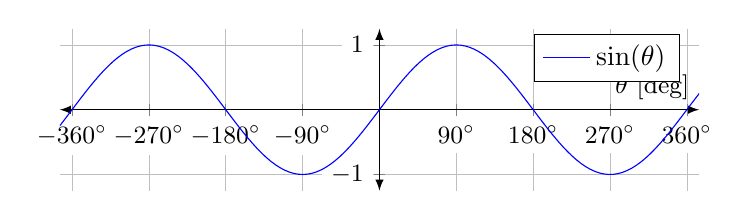
\begin{tikzpicture}
		\begin{axis}[
			myaxistrigfunctions,
			xmin=-2*pi, 
			xmax=2*pi,
			xtick={-2*pi, -3*pi/2, -pi, -pi/2, 0, pi/2, pi, 3*pi/2, 2*pi},
			xticklabels={$-360^{\circ}$, $-270^{\circ}$, $-180^{\circ}$, $-90^{\circ}$, $0$, $90^{\circ}$, $180^{\circ}$, $270^{\circ}$, $360^{\circ}$},
			domain=-3*pi:3*pi,
			samples=200,
			legend entries={$\sin(\theta)$},
			legend pos=north east,
		]
			\addplot[blue] {sin(deg(x))};
		\end{axis}
	\end{tikzpicture}
\end{solution}

\appenddata{questionSolutions}{
{
See notes
}
}